\chapter{Chapter 1 Appendix -- Focusing Provider Attention} \label{app_cc}

\section{Pilot Study (2017)} \label{app_cc_pilot}
\subsection{Pilot Study Description}
In August 2017, VaxCare piloted a program aimed at increasing influenza vaccination in their clinic partners. This pilot program launched in the state of Florida and 101 clinics were recruited to participate for the 2017 flu vaccination season. The VaxCare program direction selected the treated clinics based on clinic history. Outside of the program, 68 other Florida clinics served as a control group. 

Two elements comprised the pilot program: Financial rebates (or incentives) and performance rankings. For the rebate component, VaxCare paid a rebate of \$1, \$2, or \$3 per shot for achieving various targets of flu shot growth. VaxCare set the three rebates to correspond to three tiers of Year-over-Year flu shot growth percentages. The second-tier threshold was typically 30\% Year-over-Year growth. Earned bonuses paid out at the end of the season. This incentive structure is similar to the Medicare penalties for poor performing clinics that accompanied the Affordable Care Act \citep[see][for discussion]{Zhang2016}. For the ranking component, VaxCare ranked the participating clinics based on their flu shot growth percentage and provided these as anonymous rankings to the clinics. Clinics could access both their progress to each incentive tier and their ranking information via a web portal.

Though extensive in its setup, the pilot study still suffered from potential selection bias: Clinics who agreed to participate likely had the most to gain from participating. Despite this limitation, our analysis of the pilot study directly informed the design of the field experiment in 2018, particularly the clinic consideration criteria. 

\subsection{Results: Percent Growth and Cumulative Shots}
By the end of the study, approximately a third of the 101 treated clinics reached some level of the incentive threshold: 63 clinics did not achieve any Tier; 3 clinics achieved Tier 1 (\$1 rebate per shot); 3 clinics achieved Tier 2 (\$2 rebate per shot); and 32 achieved Tier 3 (\$3 rebate per shot). Table \ref{tab:avg_diff} details the change in flu shots for clinics in the pilot study (“treated” clinics) versus the other clinics in Florida. The net effect of the study was a 33.54\% difference in flu shots between treatment and control. 

To test the statistical significance of this result, we ran a pooled Ordinary Least Squares model on clinic cumulative flu shots (\textit{CumShots}, specification below). The Treated indicator is set to 1 for the pilot study clinics and a 0 otherwise. The coefficient $\alpha_1$ captures the treatment effect and idiosyncratic shocks are captured in $\epsilon$. From Table \ref{tab:avg_diff}, we see that the clinics in the pilot study cumulatively administered 61.8 more shots than other Florida clinics outside the study ($p < 0.01$). Altogether, we find a positive outcome: Clinics in the pilot study increased their flu shots given between 2016 and 2017.

 \begin{table}
  \resizebox{.8\textwidth}{!}{ 
  \begin{threeparttable}[t]
   \centering
   \caption{Clinic Response to “Artificial” Ranks for Rebate and Control Groups}
    \begin{tabular}{lccccc}
          & \textbf{No. Clinics} & \multicolumn{2}{c}{\textbf{No. Flu Shots}} & \textbf{Pct. Growth} & \textbf{Net Effect} \\
          &       & \textbf{2016} & \textbf{2017} &       &  \\
    Control Clinics & 68    & 10,947 & 9,933 & -9.26\% &  \\
    Treated Clinics & 101   & 22,295 & 27,707 & 24.27\% & 33.54\% \\
    \end{tabular}%
    \medskip
    % \begin{tablenotes}
    %   \footnotesize
    %   \item \textbf{Table Note:} Clinic-robust standard errors in parentheses. All models include week fixed effects. 
    %   \item (*** $p < 0.01$, ** $p < 0.05$, + $p < 0.1$)
    % \end{tablenotes}
  \label{tab:net_effect}
  \end{threeparttable} }
 \end{table}

 \begin{equation} %\begin{split} %\end{split} 
       CumShots_{it} = \alpha_0 + \alpha_1 \mathbbm{1}\{TreatedClinic\}_{i} + \epsilon_{it}
 \end{equation} 

 \begin{table}
  \resizebox{.3\textwidth}{!}{ 
  \begin{threeparttable}[t]
   \centering
   \caption{Average Difference in Cumulative Shots for Treated Pilot Study Clinics}
    \begin{tabular}{lc}
          & (1) \\
          & \textbf{CumSPP} \\
          &  \\
    Treatment Effect ($\alpha_1$) & 61.8*** \\
          & (20.23) \\
          & [0.003] \\
          &  \\
    Observations & 3718 \\
    \# clinics & 169 \\
    \end{tabular}%
    \medskip
    \begin{tablenotes}
      \footnotesize
      \item \textbf{Table Note:} Table reports standard errors clustered by clinic (surrounded by parentheses) and two-sided p values [surrounded by brackets]. 
      \item (*** $p < 0.01$, ** $p < 0.05$, + $p < 0.1$)
    \end{tablenotes}
  \label{tab:avg_diff}
  \end{threeparttable} }
 \end{table}

\subsection{Pilot Study: Limitations}
The lack of random assignment represents the primary limitation of the pilot study. VaxCare’s goal for the pilot was to find clinics that would be willing to participate As such, growing clinics might have been more willing to participate and the clinics left out of the program might not serve as a valid control group. Separately, the design of the study highlights other limitations. For example, VaxCare added several of these treated clinics as partners late in the 2016 vaccination season. Establishing a baseline for these clinics meant estimating their vaccination history. Because of the subjective nature of this estimation, the Year-over-Year percent growth goals were not uniform across all the pilot study clinics. Finally, the treated clinics simultaneously received both the financial incentives and performance feedback. We do not know which treatment ultimately led to vaccination improvement – we only know that something did. Despite these limitations, the pilot study provided an initial exploration of the impact of financial incentives and rankings on vaccinations. The study also provided important inputs for the field experiment, including randomization. The following Appendix (Section \ref{app_exp_design}) discusses these inputs and how each informed our experimental design. 


\section{Field Experiment Design (2018)} \label{app_exp_design}
\subsection{Field Experiment: Design Considerations}
Informed by these outcomes from the pilot study, we worked with VaxCare to design and launch Compliance Care in 2018. This study included 145 clinics in 9 different states. Within each state, participant clinics were identified and then randomly assigned into three treatment arms: Rebate (49 clinics), Ranking (47 clinics), and Control (49 clinics). To accomplish this, we took the following steps. 

First, to determine the necessary sample size for our experiment, we performed a power analysis using the pilot study outcomes [$(\alpha,\beta)$ set at (0.05, 0.2)]. We calculated this value assuming a case where the control clinics exceed the performance of the treated clinics to be equivalent to “no effect of the treatment” using a one-tailed t-test. Our power analysis generated a required sample size of at least 42 control clinics and 44 clinics in each treatment arm. To ensure sufficient power to detect an effect, we rounded these counts up to 50 clinics in each group (150 clinics total).

Second, we worked closely with VaxCare to implement the clinic selection and randomization process. The baseline consideration criteria were the following: We only considered Family Practice or Internal Medicine clinics; to prevent spillover, the clinics could not have participated in the pilot study; to ensure an accurate baseline for performance, the clinic was required to be a VaxCare partner for the full 2017 flu vaccine season; and finally, to verify clinic ability and commitment to administering flu shots, the clinic had to have administered at least 150 flu shots during the 2017 flu shot season. 

Third, given these consideration criteria, VaxCare selected 9 states to serve as strata; within each state, VaxCare could then randomly assigned clinics to groups. Based on each state’s overall size, VaxCare set a target number of clinics for each state. The Compliance Care leadership team then solicited the state-level salesforce for recommendations on which clinics would be representative participants while still meeting the consideration criteria; this filtered out unresponsive or uncooperative partners. This group of clinics was then randomly sorted into treatment and control groups at the state-level. Finally, given each clinic’s assigned arm, the state-level representatives solicited each clinic’s participation; though participation required no additional cost on the part of the clinic, VaxCare insisted on receiving clinic consent. With this agreement in hand, Compliance Care commenced in August 2018. Please see Figure \ref{fig:exp_timeline} for the timing of these steps and the flu shot patterns for each group during the 2018 flu vaccine season. 

Given this approach, the field experiment addresses all the concerns of the pilot study. First, we applied strict selection criteria to establish a uniform assortment of clinics. This eliminated the requirement to estimate vaccination history and enabled robust measures of clinic performance. Second, the random assignment of geographically dispersed clinics mitigates the concern of selection bias due to either performance history or location. Third, our setup included the creation of a distinct, comparable control group, instead of using screened-out clinics as a proxy for a control. Fourth, separating the treatments (financial incentives and performance feedback) for each treatment group enables independent comparison between treatment and control and between treatments. Fifth, in the Rebate group, all clinics received identical incentive thresholds (10\%/15\%/20\% Year-over-Year growth). Finally, email notifications reduced the clinical burden to checking vaccination. In summary, the field experiment permits a robust evaluation of a flu shot intervention and builds on the initial findings of the pilot study. 

 \begin{figure}[htbp]
     \centering
     \caption{Experiment Timeline \& Weekly Flu Shots by Group} %\medskip
     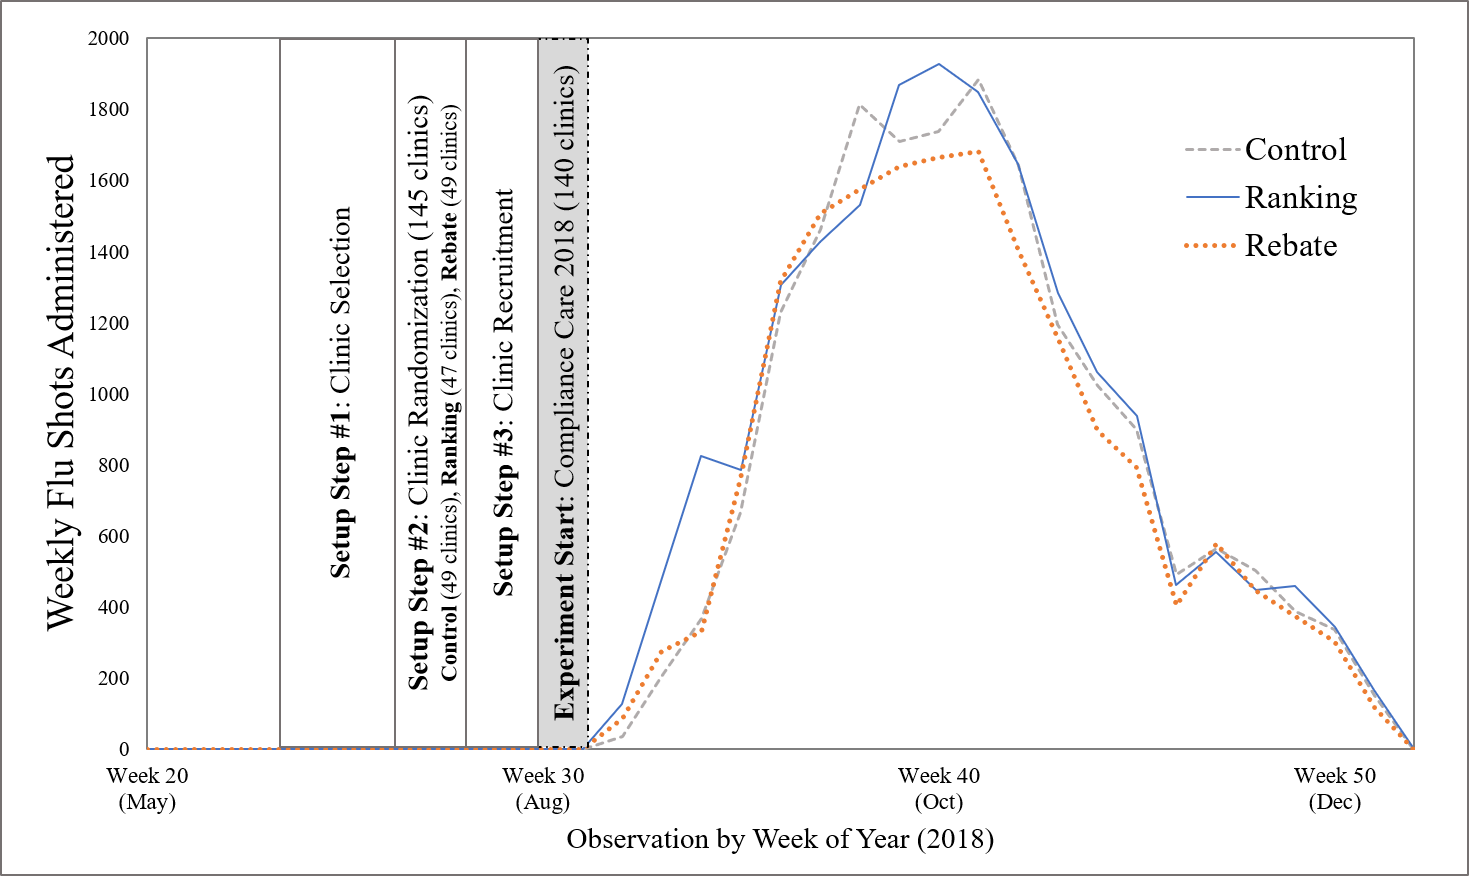
\includegraphics[scale=0.6]{Figures/CC/Figure B.1 - Experiment Timeline and Weekly Flu Shots by Group.png}     
     \label{fig:exp_timeline}
    %  \floatfoot{\textbf{Figure Note:}}
 \end{figure} 

\subsection{Field Experiment: Treatment Specifics}
As mentioned in Section \ref{cc_setup}, the treated clinics received an automated email each week from VaxCare. During the clinic recruitment phase, each clinic identified a staff member to VaxCare to serve as the point person for the program. In some cases, clinics identified their office manager as the point person, while in other cases, clinics selected a senior medical assistant who oversaw the clinic vaccination process. In any case, this point person served as the primary correspondent during the experiment while the clinic’s physicians received a carbon-copy of these reports as well. During recruitment, VaxCare carefully explained the format of these weekly emails, and clinics were encouraged to contact VaxCare’s customer care team with any follow-on questions. Based on our survey of these clinics, we know the contents of this email were reviewed regularly and shared generally with the rest of the staff – for example, at a weekly staff meeting. 

These emails contained the following elements. At the very top, the emails prominently highlighted each clinics’ specific treatment information, either flu shot percent growth or clinic rank. Next, clinics in both treatments received a growth table which outlined how many clinics shots were given by month either in 2017 (prior to the intervention) or in 2018 (during the intervention). Finally, the emails to the Rebate clinics also contained each vaccination threshold which corresponded to each of the three incentive tiers. For example, a clinic that administered 360 shots by the end of 2017 (as displayed in the growth table) would receive a Tier 1 threshold set at 396 shots corresponding to 10\% growth. The Rebate clinics received tiered incentive thresholds with rebates of \$1, \$2, and \$3 per shot awarded for achieving the targets set at 10\%, 15\%, and 20\% Year-over-Year flu shot growth. Rebate clinics who surpassed the tiered thresholds received that tier’s rebates for all shots given, including shots given before surpassing the threshold.


\section{Sensitivity and Test of Randomization} \label{app_cc_sens}
“The most credible and influential research designs use random assignment” \citep[p. 11]{Angrist2009}. Though ubiquitous in medicine, the Randomized Controlled Trial (RCT) has become more common in many academic disciplines, including economics, social science, and operations. And yet, even the “gold standard” of causal inference is not without assumptions. The purpose of this Appendix is to acknowledge any limitations and provide evidence that the findings presented in the remainder of the paper can still be considered valid. We refer interested readers to an extensive discussion of the limits of RCTs presented in \cite{Deaton2018}. 

As detailed in \cite{Deaton2018}, in order to estimate an unbiased average treatment effect (ATE), the researcher must assume balance between treated and non-treated subjects (or clinics). Proper randomization provides this balance in expectation \citep[p. 4]{Deaton2018}, assuming an infinite sample and an infinite number of randomizations. Practically, it is impossible to perform an infinite number of randomizations among an infinite sample, and any actual RCT must accept this as a limitation – that the estimated ATE is only unbiased in expectation. Researchers can, however, test for balance among observable covariates. 

Unfortunately, finding balance in observed covariates does not guarantee overall balance; the nature of unobserved covariates is just that – they are unobserved, and if any of these features are unbalanced and correlate with the treatment then the estimate of the ATE will in fact be biased. Thus, the previous assumption evolves to the following: If we can demonstrate balance in the observed covariates, then we argue that the likelihood is high that we have also achieved balance in the unobserved covariates leading to an unbiased estimate. This is akin to an assumption of unconfoundedness in the treatment effects literature \citep[e.g.,][]{Rubin1990} or more generally as the \cite{Heckman1985} assumption of selection on observables. The remainder of this addendum evaluates the balance between the Control, Ranking, and Rebate groups. Our analyses in this appendix can be \textbf{summarized} as follows: \\
1.	We cannot reject individual balance between means of 21 covariates for all 3 clinic groupings. \\
2.	We cannot reject joint balance between means of 21 covariates for all 3 clinic groupings.\\
3.	Without any further action (i.e., before trimming), we demonstrate acceptable common support in clinic treatment propensity as determined by 8 covariates. Only 3 clinics exhibit propensities outside of this support.\\
4.	After trimming these 3 clinics, and one additional clinic which lacks a comparison in the same state, we demonstrate excellent common support in clinic treatment propensity as determined by the same 8 covariates. We proceed to use this smaller clinic subset for two further tests.\\
5.	\textbf{Test 1}: When matching treated (Ranking/Rebate) to control clinics using the same 8 covariates, we see results in-line with our previous analyses: The Ranking clinics increase their flu shots by 15.8\% more than their matched Control clinics, and the result is statistically significant ($p < 0.05$). We also find no statistically significant effect between the Rebate clinics and their matched Control clinics.\\
6.	\textbf{Test 2}: After evaluating our panel regression models for clinic Percent Growth in flu shots (Specification 1) and clinic Shots per Patient-Population (Specification 4), our results are nearly identical to our findings before trimming: We find a statistically significant ($p < 0.05$) and similarly sized treatment effect for both outcome variables.\\

As a result, given that: (1) we cannot reject balance among our observable clinic measures; (2) we demonstrate that our clinics have common support; (3) we highlight the performance gap between Ranking and matched Control clinics which is consistent with our initial findings; and (4) our primary regression models are not sensitive to the inclusion or removal of clinics who lack common support; we conclude that we have demonstrated balance among our clinic groups and our treatment effect is unlikely to be biased. Nevertheless, we conservatively exclude these 4 clinics from our results which compare clinics between different groups.

\subsection{Test of Clinic Profiles: t-Test of clinic means}
As a first step, we want to rule out the possibility of differences in clinic profiles driving our results. To test these clinic profiles, we performed ‘t-Tests’ on the equality of the following variables between groups (Control versus Ranking, Ranking versus Rebate, and Control versus Rebate). The result of this operation is 63 total t-Tests (21 variables tested for 3 group comparisons). Here, we are testing the null hypothesis that these clinic profiles are the same in each of these categories. We restrict these comparisons to the clinics who completed the season as VaxCare partners. 

\begin{table}[htbp]
\resizebox{1\textwidth}{!}{ 
  \centering
  \caption{Variables Tested: t-Test, Hotelling’s T$^2$ Generalized Means Test}
    \begin{tabular}{ll}
    \textbf{2017 Variables} & \textbf{2018 Variables} \\
    Clinic: Percent Male Patients in 2017 & Clinic: Percent Male Patients in 2018 \\
    Clinic: Percent Patients over 65 in 2017 & Clinic: Percent Patients over 65 in 2018 \\
    Clinic: Average Patient Age in 2017 & Clinic: Average Patient Age in 2018 \\
    Clinic: Percent Medicare Patients in 2017 & Clinic: Percent Medicare Patients in 2018 \\
    Clinic: Percent Comm. Insurance Patients in 2017 & Clinic: Percent Comm. Insurance Patients in 2018 \\
    Clinic MD Count in 2017 & Clinic MD Count in 2018 \\
    Clinic Patient Count, Flu Shot Season 2017 & Clinic Patient Count, Flu Shot Season 2018 \\
          & Patient Count Difference, Flu Shot Season, 2017 to 2018 \\
    Clinic Patient Count, all of 2017 & Clinic Patient Count, all of 2018 \\
    Clinic: Flu Shot Total in 2017 & Clinic: Flu Shot Total in 2018 \\
    Clinic: Shots per Patient in 2017 & Clinic: Shots per Patient in 2018 \\
    \end{tabular}% 
  \label{tab:var_test} }
\end{table}%

The conclusion of these tests is that we cannot reject the null in 62 out of 63 tests ($p > 0.05$). The only test that rejects this null ($p < 0.05$) is the comparison for clinic percent of male patients between the Control and Rebate group in 2017. This rate is not greater than chance: With 63 tests we would expect a little over 3 of these tests to fail on average. As such, we claim balance on these observable covariates between all 3 groups.

\subsection{Test of Clinic Profiles: Hotelling’s T-squared generalized means test}
The previous test performs an individual test for each variable, but we can also test these equalities jointly. To do this, we performed “Hotelling’s T-squared generalized means test” to jointly compare the means of all above variables between the three groups \citep{Hotelling1931}. In this case, we cannot reject any of the null hypotheses that these groups are statistically equivalent ($p > 0.15$).

\subsection{Test of Clinic Profiles: Propensity to Treatment}
As a final test of the similarity of clinic profiles, we can calculate the propensity to being included as a treated clinic instead of a control clinic. We use this method to demonstrate that our treated (Ranking/Rebate) and control clinics share common support. The issue surrounding common support is discussed widely in the treatment effects literature; we refer readers to seminal papers in \cite{Caliendo2008} and \cite{Stuart2010}. 

Provided we can demonstrate we have common support between our treated and control clinics, our previous argument holds: Common support (or balance) in observed covariates increased the likelihood of common support in unobserved covariates, and we can compare groups to evaluate the effect of our treatment.

\subsection*{Evaluation of Common Support} 
In line with the treatment effects literature, we calculate each clinic’s propensity to be included as a treated clinic with a logistic regression model. The choice of included variables requires researcher discretion, but in line with \cite{Caliendo2008} and \cite{Angrist2009}, we choose variables that might simultaneously influence inclusion into the study and the treatment outcome. As such, we include the eight clinic-level variables listed in Table \ref{tab:var_input}. 

\begin{table}[htbp]
\resizebox{1\textwidth}{!}{ 
  \centering
  \caption{Variable Inputs: Evaluating Common Support \& Matching Outcomes}
    \begin{tabular}{lr}
    \textbf{2017 Variables} & \multicolumn{1}{l}{\textbf{2018 Variables}} \\
    Clinic MD Count in 2017 & \multicolumn{1}{l}{Clinic MD Count in 2018} \\
    Clinic Patient Count, Flu Shot Season 2017 & \multicolumn{1}{l}{Clinic Patient Count, Flu Shot Season 2018} \\
          & \multicolumn{1}{l}{Patient Count Difference, Flu Shot Season, 2017 to 2018} \\
    Clinic Patient Count, all of 2017 & \multicolumn{1}{l}{Clinic Patient Count, all of 2018} \\
    Clinic: Flu Shot Total in 2017 &  \\
    Clinic: Shots per Patient in 2017 &  \\
    \end{tabular}%
  \label{tab:var_input} } %
\end{table}%

We omit the demographic variables (e.g., percent male patients) as we do not have reason to believe these variables affected our outcome and they were not considered in our clinic consideration criteria. We do not include potential outcome measures (e.g., clinic shots per patient population in 2018), as the treated clinics had the opportunity to affect these outcomes. As in our main analysis, we restrict this analysis to clinics that started the vaccination season as VaxCare partners (N = 140). The following charts display the kernel density of the calculated propensities, both before and after trimming.

 \begin{figure}
     \centering
     \caption{Propensity to Treatment: Common Support Before Trimming} %\medskip
     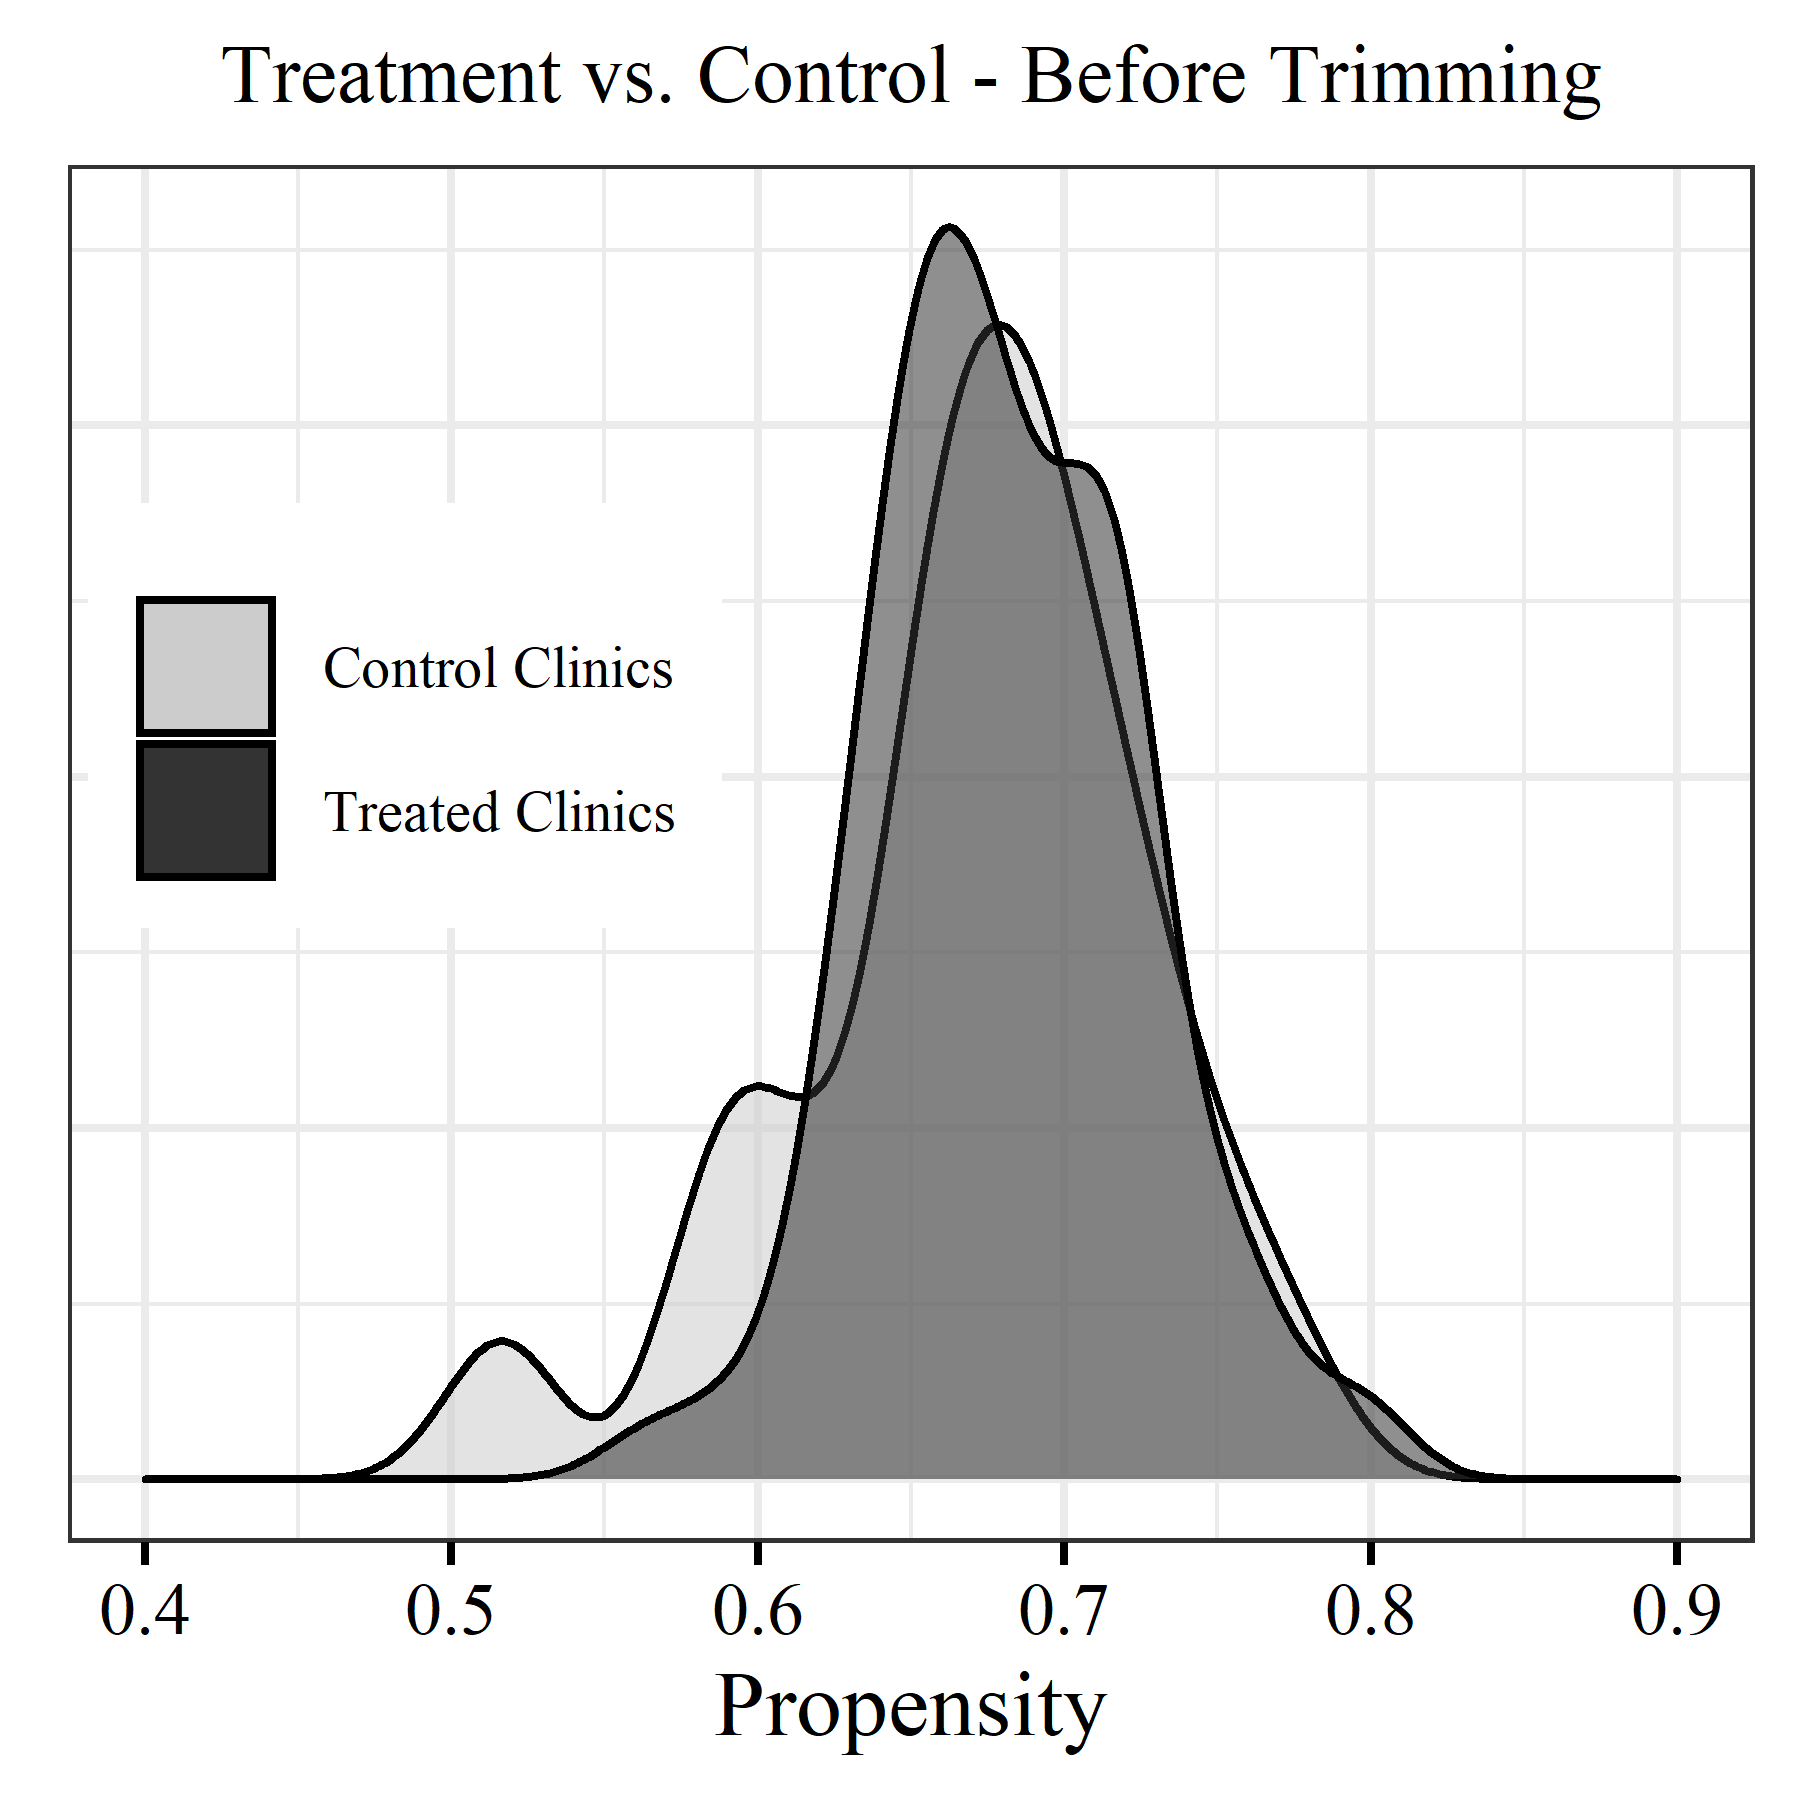
\includegraphics[scale=1]{Figures/CC/Figure C.1 (left).png}     
     \label{fig:pre_trim}
    %  \floatfoot{\textbf{Figure Note:}}
 \end{figure}  
 \begin{figure}
     \centering
     \caption{Propensity to Treatment: Common Support After Trimming} %\medskip
     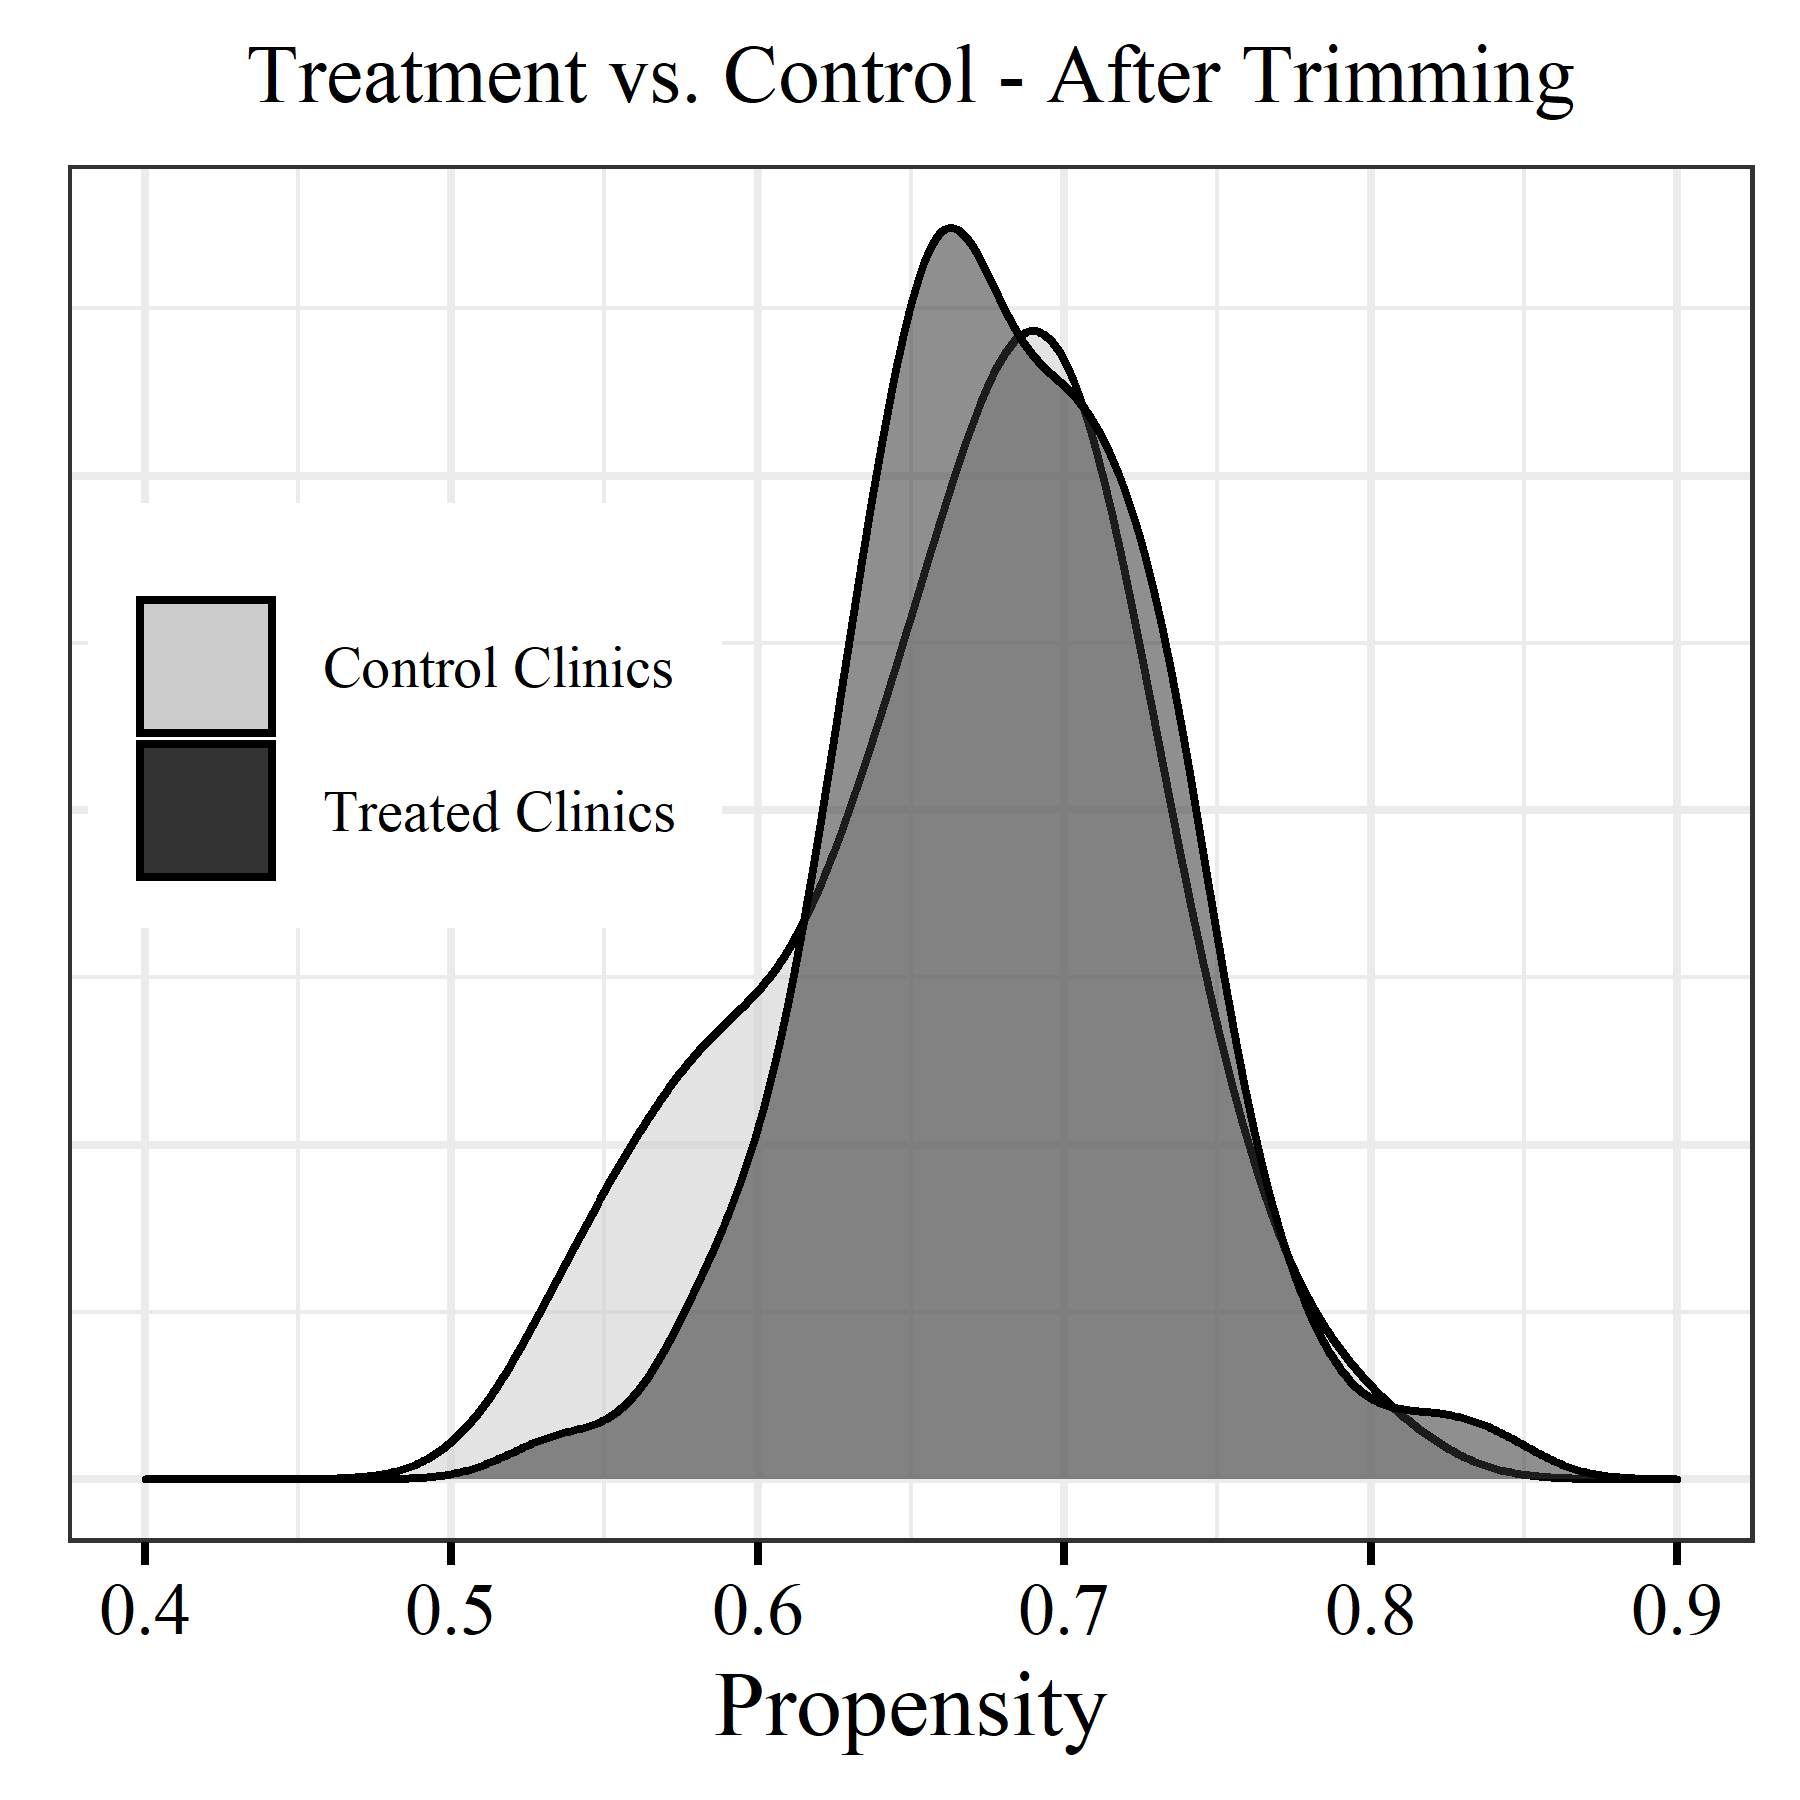
\includegraphics[scale=1]{Figures/CC/Figure C.1 (right).png}     
     \label{fig:post_trim}
    %  \floatfoot{\textbf{Figure Note:}}
 \end{figure} 

Figure \ref{fig:pre_trim} illustrates that there is common support for many of our clinics, even before trimming; there is significant overlap in the right-hand portion of the density graph. Nevertheless, there is one control clinic and two treated clinics with low propensity scores (less than 0.5) that have no comparable clinics. As these clinics do not possess comparable inputs, we should consider excluding them from our analysis. By dropping these clinics, we compromise our sample size but can more reasonably conclude that we are comparing similar clinics to one another. After dropping these three clinics, we are left with only one clinic in South Carolina. Our randomization was stratified by state, and as this clinic no longer has a comparable clinic in the state, the conservative approach is to also drop this clinic. 

After trimming these clinics, we recalculate our propensity to treatment, and this gives the density graph in Figure \ref{fig:post_trim}. As a result, we can reasonably conclude that we have common support for the above variables between our treated and our control clinics. Our final clinic distribution can be seen in Table \ref{tab:clinic_dist}. We proceed to evaluate the robustness of our outcomes to excluding these 4 clinics.

\begin{table}[htbp]
\resizebox{1\textwidth}{!}{ 
  \centering
  \caption{Average Treatment Effect for Matched Ranking and Rebate Clinics}
    \begin{tabular}{lcccc}
    \textbf{Treatment Group} & \textbf{Clinic Partners} & \textbf{Propensity Exclusion} & \textbf{State Exclusion} & \textbf{Final Clinic Count} \\
    Control & 46    & 1     & 1     & 44 \\
    Ranking & 46    & 2     & -     & 44 \\
    Rebate & 48    & -     & -     & 48 \\
    Clinic Total & 140   &       &       & 136 \\
    \end{tabular}%
  \label{tab:clinic_dist} } %
\end{table}%

\subsection*{Robustness Test 1: Matched Clinics} 
After excluding the four clinics above, we perform a test using a nearest neighbor matching method. This method is formally detailed in \cite{Abadie2006} with amplification in \cite{Abadie2011}. In short, nearest neighbor matching first determines the nearest neighbor using a weighted function of inputs. Once this neighbor is identified, the missing potential outcome is imputed by using the realized outcome of the nearest neighbor. The average treatment effect (ATE) is the average of the difference between realized and imputed outcomes for each clinic.

We match clinics and evaluate the outcome at the conclusion of our study. Starting with the Ranking clinics, we use the same eight variables listed in the previous table as inputs to match these clinics to the nearest, comparable Control clinics. We then do the same for the Rebate clinics. We also apply the bias adjustment for the continuous variables as discussed in \cite{Abadie2011}. Because patient counts, changes in patient count, and total doses serve to match these clinics, we test a separate, outcome independent of these factors: Year-over-Year percent growth in flu shots between 2017 and 2018. 

\begin{table}[htbp]
\resizebox{1\textwidth}{!}{ 
  \centering
  \caption{Average Treatment Effect for Matched Ranking and Rebate Clinics}
    \begin{tabular}{cccccc}
    \textbf{Treatment} & \textbf{Outcome} & \textbf{No. of observations} & \textbf{ATE} & \textbf{Standard error} & \textbf{Significance} \\
    Ranking & YoY Percent Growth & 44+44 = 88 & 0.158 & 0.0687 & $p < 0.05$ \\
    Rebate & YoY Percent Growth & 44+48 = 92 & 0.00152 & 0.0908 & $p > 0.10$ \\
    \end{tabular}%
  \label{tab:avg_te_2} } %
\end{table}%

After matching, the Rebate clinics show no statistically significant difference from their matched Control clinics, in line with our previous findings. For the Ranking clinics, however, we do see a statistically significant treatment effect: The Ranking clinics grew flu shots by 15.8\% more than their matched Control clinics. The magnitude of this effect is even more noteworthy, as only one comparison is made at the end of the year, whereas Specification 1 and Specification 4 evaluate the cumulative impact of the treatment over the entire season. We proceed to evaluate our regression models while only including the clinics with common support.

\subsection*{Robustness Test 2: Random Effects Regression Models} 
After excluding the clinics without common support, we are left with 136 clinics. We proceed to test the sensitivity of our findings to including or excluding the 4 clinics without common support. We tested our primary outcome measure (weekly percent growth of clinics over the 2018 vaccination season, or \textit{PercentGrowth} from Section \ref{emp_spec_pctGrowth}) and our alternate outcome measure (Cumulative Shots per Patient-Population, or \textit{CumSPP} from Section \ref{app_cc_alt_dv}). The econometric specifications follow the main text, and we continue to cluster the errors at the clinic level.
  \begin{equation} \tag{1} %\begin{split} %\end{split} 
      PercentGrowth_{it} = \beta_0 + \beta_1 TreatmentGroup_i + ClinicState_i + PatientCount_i + \epsilon_{it} 
  \end{equation}
  \begin{equation} \tag{4} \begin{split}
       CumSPP{it} = \beta_0 & + \beta_1 TreatmentGroup_i \times Year_t \\
       & + Year_t + TreatmentGroup_i \\ & + ClinicState_i + ClinicState_i \times Year_t + \epsilon_{it} 
  \end{split}  \end{equation}
  

Table \ref{tab:te_w_cs} presents the results of these regressions. Our results from Section \ref{cc_res_pctGrowth} (Specification 1) and Section \ref{app_cc_alt_dv} (Specification 4) are included in Columns 1 and 3 for comparison. The results from Column 2 show, on average, the Ranking clinics grew by approximately 7.9\% more than the Control clinics ($p < 0.05$) while the Rebate clinics show no meaningful difference in growth from the control. Furthermore, the results from Column 3 for Shots per Patient-Population show, on average, the Ranking clinics vaccinated 4.6\% more of their respective patient population than the Control clinics while the Rebate clinics show no meaningful difference. These results are nearly identical, though with slightly less precision in the smaller clinic sample. 

Given the results of both tests, along with our verification of common support, we conclude that we do have balance in our groups and our treatment effects are not sensitive to clinic profiles, affirming the validity and robustness of our randomization efforts. 

 \begin{table}
  \resizebox{1\textwidth}{!}{ 
  \begin{threeparttable}[t]
   \centering
   \caption{Treatment Effect of Compliance Care on Clinics with Common Support}
    \begin{tabular}{lcccc}
          & (1)   & (2)   & (3)   & (4) \\
          & \textbf{Percent Growth} & \textbf{Percent Growth} & \textbf{Shots per Patient Population } & \textbf{Shots per Patient Population } \\
    Econometric Model & Specification 1 & Specification 1 & Specification 4 & Specification 4 \\
          &       &       &       &  \\
    Ranking (Post-Treatment) & 0.0833** & 0.0793** & 0.0459** & 0.0460** \\
          & (0.0406) & (0.0395) & (0.0232) & (0.0224) \\
    Rebate (Post-Treatment) & 0.00219 & 0.00398 & 0.0125 & 0.0127 \\
          & (0.0399) & (0.0396) & (0.0235) & (0.0231) \\
          &       &       &       &  \\
    Observations & 2,720 & 2,800 & 5,712 & 5,880 \\
    \# clinics & 136   & 140   & 136   & 140 \\
    \end{tabular}%
    \medskip
    \begin{tablenotes}
      \footnotesize
      \item \textbf{Table Note:} Robust standard errors, clustered by clinic, in parentheses. Specification 1 includes clinic patient count and clinic state fixed effects. Specification 4 includes a year fixed effect, a state fixed effect, and an interaction between clinic state and year. 
      \item (*** $p < 0.01$, ** $p < 0.05$, + $p < 0.1$)
    \end{tablenotes}
  \label{tab:te_w_cs}
  \end{threeparttable} }
 \end{table}


\section{Alternate Dependent Variable} \label{app_cc_alt_dv}
When comparing clinic outcomes during Compliance Care, one must remember that clinics vary in size and capacity to deliver flu shots. Some clinics can administer 2,000 flu shots in a flu season, while others might only deliver 200 shots. Our primary dependent variable accounts for these factors by normalizing for Year-over-Year flu shot percent growth. As an alternate approach, we divide the cumulative number of weekly flu shots given by each clinics’ total patient population over the vaccination season (all patients who sought any clinic service) - Shots per Patient-Population. This metric addresses this consideration by normalizing by patient volume for large and small clinics. In line with a difference-in-differences approach, we interact a factor variable for treatment with an indicator variable for year. The resulting output measures the difference between the groups by year.  
  \begin{equation} \tag{4} \begin{split}
       CumSPP{it} = \beta_0 & + \beta_1 TreatmentGroup_i \times Year_t \\
       & + Year_t + TreatmentGroup_i \\ & + ClinicState_i + ClinicState_i \times Year_t + \epsilon_{it} 
  \end{split}  \end{equation}

We present the resulting Cumulative Shots per Patient-Population ($CumSPP$) for clinic $i$ in week $t$. The $TreatmentGroup$ variable is a factor variable with a level for each treatment (Control/Ranking/Rebate). The coefficient on the interaction variable specifies the performance difference between groups between 2017 and 2018. The $Year$ variable controls for the differing time trend between 2017 and 2018. We also include a state fixed effect and an interaction between Year and State to control for differing demand patterns in each geographic region each year. The idiosyncratic shocks which we have not controlled for are captured in $\epsilon$. 

As in Section \ref{cc_res_comp}, we conservatively focus on the clinics with common support (N = 136). The results of Table \ref{tab:te_alt_dv} show, on average, the Ranking clinics vaccinated approximately 5\% more of their respective patient population than the Control clinics while the Rebate clinics show no meaningful difference. As above, it appears the Ranking group outperformed the Control and the Rebate group. A Wald test confirms this by rejecting the null hypothesis that the Rebate clinics outperformed the Ranking clinics ($\beta_{1,rebate} >= \beta_{1,ranking}$; $p = 0.051$). Given this outcome and the outcome of Section \ref{cc_res_comp}, we confidently reject Hypothesis 1a and Hypothesis 2.

 \begin{table}
  \resizebox{0.5\textwidth}{!}{ 
  \begin{threeparttable}[t]
   \centering
   \caption{Treatment Effect of Compliance Care on Shots per Patient-Population (SPP)}
    \begin{tabular}{lc}
          & (1) \\
          & \textbf{Shots per Patient Population} \\
          &  \\
    Ranking (Post-Treatment) & 0.0459** \\
          & (0.0232) \\
    Rebate (Post-Treatment) & 0.0125 \\
          & (0.0235) \\
          &  \\
    Observations & 5,712 \\
    \# clinics & 136 \\
    \end{tabular}%
    \medskip
    \begin{tablenotes}
      \footnotesize
      \item \textbf{Table Note:} Robust standard errors, clustered by clinic, in parentheses. Model also includes a year fixed effect, a state fixed effect, and an interaction between clinic state and year fixed effect. 
      \item (*** $p < 0.01$, ** $p < 0.05$, + $p < 0.1$)
    \end{tablenotes}
  \label{tab:te_alt_dv}
  \end{threeparttable} }
 \end{table}

\section{Rank Response Sensitivity Analysis} \label{app_cc_rankResp_sens}
Given the results of Specification 3 in Section \ref{cc_res_rankResp}, we proceed to test the sensitivity of our conclusions for various definitions of first and last place. To evaluate our thresholds, we fix one parameter at the original definition and vary the other. For example, we reserve the high rank flag for clinics ranked in the top 5 but then relax and restrict the threshold for the bottom ranked clinics to test Last-Place Aversion. This test will also confirm or deny our lack of evidence for First-Place Loving behavior in the previous analysis (Section \ref{cc_res_rankResp}). We use the same outcome variable as defined in Section \ref{emp_spec_pctGrowth} (weekly shots per patient-population metric).

For various definitions of last place, please see Table \ref{tab:sensitivity_def_last}. We restrict our definition of last to only consider the lowest rank ($LowRank = 1$ if Rank $\in$ [46,46]) and relax our definition to consider clinics ranking in bottom 11 ranks ($LowRank = 1$ if Rank $\in$ [36,46]). We find statistically significant evidence for Last-Place Aversion even when relaxing the definition to consider clinics ranked in the bottom 10 ($p < 0.05$). Furthermore, evidence for Last-Place Aversion eventually vanishes. This is a welcome addition, as we would not expect Last-Place Aversion to exist for all definitions of last place. 

For various definitions of first place, please see Table \ref{tab:sensitivity_def_first}. We restrict our definition of first to only consider the top rank ($HighRank = 1$ if Rank $\in$ [1,1]) and relax our definition to consider the top 10 ranks ($HighRank = 1$ if Rank $\in$ [1,10]). The results are statistically significant when first place is defined as either of the top two ranks ($p < 0.01$ in Column 1 and $p < 0.10$ in Column 2); in all other definitions, the results are not statistically significant. Thus, if we restrict our definition of first place, we may have evidence of First-Place Loving behavior. However, in light of the robustness check in Section \ref{app_cc_grp_robust}, we cannot conclude this is not an artifact of some other unobservable behavior. Thus, we conclude that we do not have sufficient evidence to identify First-Place Loving behavior.

In summary, we find (1) our findings for First-Place Loving behavior are sensitive to our definition of “first” place and (2) our findings for Last-Place Aversion are not sensitive to our definition of “last place.” Thus, we find increasing evidence in support of Hypothesis 4. 

 \begin{table}
  \resizebox{1\textwidth}{!}{ 
  \begin{threeparttable}[t]
   \centering
   \caption{The Effect of Moving into a “Low” Rank on Weekly Shots per Patient-Population}
    \begin{tabular}{lcccccr}
          & (1)   & (2)   & (3)   & (4)   & (5)   & \multicolumn{1}{c}{(6)} \\
          & \textbf{WeekSPP} & \textbf{WeekSPP} & \textbf{WeekSPP} & \textbf{WeekSPP} & \textbf{WeekSPP} & \multicolumn{1}{c}{\textbf{WeekSPP}} \\
          &       &       &       &       &       &  \\
    Low Flag = 1 if Rank $\in$ & [36,46] & [37,46] & [38,46] & [39,46] & [40,46] & \multicolumn{1}{c}{[41,46]} \\
    Coeff.: Low Rank ($\pi_1$) & 0.00984 & 0.0136** & 0.0167*** & 0.0171*** & 0.0229*** & \multicolumn{1}{c}{0.0240***} \\
          & (0.00622) & (0.00606) & (0.00573) & (0.00596) & (0.00631) & \multicolumn{1}{c}{(0.00665)} \\
    High Flag = 1 if Rank $\in$ & [1,5] & [1,5] & [1,5] & [1,5] & [1,5] & \multicolumn{1}{c}{[1,5]} \\
    Coeff.: High Rank ($\pi_2$) & 0.00556 & 0.00557 & 0.00568 & 0.00551 & 0.00514 & \multicolumn{1}{c}{0.00517} \\
          & (0.00574) & (0.00571) & (0.00576) & (0.00579) & (0.00580) & \multicolumn{1}{c}{(0.00581)} \\
          &       &       &       &       &       &  \\
    Observations & 792   & 792   & 792   & 792   & 792   & \multicolumn{1}{c}{792} \\
    \# clinics & 46    & 46    & 46    & 46    & 46    & \multicolumn{1}{c}{46} \\
          &       &       &       &       &       &  \\
          & (7)   & (8)   & (9)   & (10)  & (11)  &  \\
          & \textbf{WeekSPP} & \textbf{WeekSPP} & \textbf{WeekSPP} & \textbf{WeekSPP} & \textbf{WeekSPP} &  \\
          &       &       &       &       &       &  \\
    Low Flag = 1 if Rank $\in$ & [42,46] & [43,46] & [44,46] & [45,46] & [46,46] &  \\
    Coeff.: Low Rank ($\pi_1$) & 0.0273*** & 0.0306*** & 0.0364*** & 0.0408*** & 0.0325*** &  \\
          & (0.00767) & (0.00936) & (0.00864) & (0.0116) & (0.00585) &  \\
    High Flag = 1 if Rank $\in$ & [1,5] & [1,5] & [1,5] & [1,5] & [1,5] &  \\
    Coeff.: High Rank ($\pi_2$) & 0.00461 & 0.00477 & 0.00480 & 0.00498 & 0.00492 &  \\
          & (0.00572) & (0.00568) & (0.00566) & (0.00562) & (0.00563) &  \\
          &       &       &       &       &       &  \\
    Observations & 792   & 792   & 792   & 792   & 792   &  \\
    \# clinics & 46    & 46    & 46    & 46    & 46    &  \\
    \end{tabular}%
    \medskip
    \begin{tablenotes}
      \footnotesize
      \item \textbf{Table Note:} This table details the specific effects of Ranking clinics moving into last place. All models include week fixed effects. Robust standard errors, clustered by clinic, in parentheses. The results from Table 2 (Column 2) have been duplicated in Column 7.
      \item (*** $p < 0.01$, ** $p < 0.05$, + $p < 0.1$)
    \end{tablenotes}
  \label{tab:sensitivity_def_last}
  \end{threeparttable} }
 \end{table}
 
  \begin{table}
  \resizebox{0.9\textwidth}{!}{ 
  \begin{threeparttable}[t]
   \centering
   \caption{The Effect of Moving into a “High” Rank on Weekly Shots per Patient-Population}
    \begin{tabular}{lccccc}
          & (1)   & (2)   & (3)   & (4)   & (5) \\
          & \textbf{WeekSPP} & \textbf{WeekSPP} & \textbf{WeekSPP} & \textbf{WeekSPP} & \textbf{WeekSPP} \\
          &       &       &       &       &  \\
    Low Flag = 1 if Rank $\in$ & [42,46] & [42,46] & [42,46] & [42,46] & [42,46] \\
    Coeff.: Low Rank ($\pi_1$) & 0.0273*** & 0.0273*** & 0.0273*** & 0.0273*** & 0.0273*** \\
          & (0.00765) & (0.00763) & (0.00767) & (0.00769) & (0.00767) \\
    High Flag = 1 if Rank $\in$ & [1,1] & [1,2] & [1,3] & [1,4] & [1,5] \\
    Coeff.: High Rank ($\pi_2$) & 0.0203*** & 0.0116+ & 0.00539 & 0.00768 & 0.00461 \\
          & (0.00687) & (0.00686) & (0.00590) & (0.00704) & (0.00572) \\
          &       &       &       &       &  \\
    Observations & 792   & 792   & 792   & 792   & 792 \\
    \# clinics & 46    & 46    & 46    & 46    & 46 \\
          &       &       &       &       &  \\
          & (6)   & (7)   & (8)   & (9)   & (10) \\
          & \textbf{WeekSPP} & \textbf{WeekSPP} & \textbf{WeekSPP} & \textbf{WeekSPP} & \textbf{WeekSPP} \\
          &       &       &       &       &  \\
    Low Flag = 1 if Rank $\in$ & [42,46] & [42,46] & [42,46] & [42,46] & [42,46] \\
    Coeff.: Low Rank ($\pi_1$) & 0.0273*** & 0.0275*** & 0.0277*** & 0.0276*** & 0.0275*** \\
          & (0.00764) & (0.00776) & (0.00780) & (0.00780) & (0.00773) \\
    High Flag = 1 if Rank $\in$ & [1,6] & [1,7] & [1,8] & [1,9] & [1,10] \\
    Coeff.: High Rank ($\pi_2$) & 0.00131 & 0.00557 & 0.00478 & 0.00480 & 0.00311 \\
          & (0.00482) & (0.00480) & (0.00449) & (0.00413) & (0.00437) \\
          &       &       &       &       &  \\
    Observations & 792   & 792   & 792   & 792   & 792 \\
    \# clinics & 46    & 46    & 46    & 46    & 46 \\
    \end{tabular}%

    \medskip
    \begin{tablenotes}
      \footnotesize
      \item \textbf{Table Note:} This table details the specific effects of Ranking clinics moving into first place. All models include week fixed effects. Robust standard errors, clustered by clinic, in parentheses.
      \item (*** $p < 0.01$, ** $p < 0.05$, + $p < 0.1$)
    \end{tablenotes}
  \label{tab:sensitivity_def_first}
  \end{threeparttable} }
 \end{table}

\newpage
\section{Rank Response – Robustness to Group Setting} \label{app_cc_grp_robust}
As discussed in Section \ref{rpf_robust}, we must consider mean reversion as an alternative mechanism for our findings. To test for this, we artificially ranked the clinics in the Control group (with respect to each other) and the clinics in the Rebate group (with respect to each other). We then applied our weekly shots per patient-population metric (defined in Section \ref{emp_spec_pctGrowth}) to the Control and Rebate clinics via Specification 2 and Specification 3, similar to a placebo test. 
\subsection{Specification 2: Results for Control and Rebate Clinics}
Table \ref{tab:art_ranks_reb_ctrl} contains the results of applying Specification 2 to the Rebate and Control groups. For the Rebate and Control group, not only are the coefficient magnitudes insignificant, but the coefficient signs are also different from the Ranking group, indicating a completely different function (i.e., not a U-shaped First-Place Loving/Last-Place Aversion curve) is (poorly) fitted to these two groups.

\begin{table}[!b]
  \resizebox{0.7\textwidth}{!}{ 
  \begin{threeparttable}[t]
   \centering
   \caption{Response to “Artificial” Ranks for Rebate and Control Groups}
    \begin{tabular}{lccc}
          & (1)   & (2)   & (3) \\
          & \textbf{WeekSPP} & \textbf{WeekSPP} & \textbf{WeekSPP} \\
          &       &       &  \\
    Clinic Group & Ranking & Rebate & Control \\
    Rank, previous week ($\lambda_1$) & -0.00209*** & 0.000867 & -0.000163 \\
          & (0.000648) & (0.000782) & (0.000940) \\
    Rank$^2$, previous week ($\lambda_2$) & 5.34e-05*** & -1.83e-05 & -4.98e-06 \\
          & (1.36e-05) & (2.10e-05) & (2.66e-05) \\
          &       &       &  \\
    Observations & 792   & 823   & 742 \\
    \# clinics & 46    & 48    & 44 \\
    \end{tabular}%
    \medskip
    \begin{tablenotes}
      \footnotesize
      \item \textbf{Table Note:} This table the parameter estimates from Model 2 for all clinic groups: Ranking, Rebate, and Control. Robust standard errors, clustered by clinic, in parentheses. All models include week fixed effects. 
      \item (*** $p < 0.01$, ** $p < 0.05$, + $p < 0.1$)
    \end{tablenotes}
  \label{tab:art_ranks_reb_ctrl}
  \end{threeparttable} }
 \end{table}

\subsection{Specification 3: Results for Control Clinics}
When testing for Last-Place Aversion, we test any definition of last place down to clinics that were ranked in the bottom half (ranks greater than or equal to 23 out of 46 Control clinics). In this case, we do not see any statistically significant results among the Control clinics for any of these definitions for Model 3. When testing for First-Place Loving behavior, we test for all definitions of first place to clinics ranked in the top 10; we do see instances of statistically significant results in the top ranks (Columns 1, 2 and 3 under Table \ref{tab:move_high_rank}). For example, when defining “first” as the top rank only, the control clinics respond to non-existent ranks with a +1.21\% change in shots per patient-population ($p < 0.05$). 

\begin{table} %[!b]
  \resizebox{0.9\textwidth}{!}{ 
  \begin{threeparttable}[t]
   \centering
   \caption{The Effect of Moving into a “High” Rank on Weekly Shots per Patient-Population}
    \begin{tabular}{lccccc}
          & (1)   & (2)   & (3)   & (4)   & (5) \\
          & \textbf{WeekSPP} & \textbf{WeekSPP} & \textbf{WeekSPP} & \textbf{WeekSPP} & \textbf{WeekSPP} \\
    Clinic Group & Control & Control & Control & Control & Control \\
    Econometric Model & Specification 3 & Specification 3 & Specification 3 & Specification 3 & Specification 3 \\
          &       &       &       &       &  \\
    High Flag = 1 if Rank $\in$ & [1,1] & [1,2] & [1,3] & [1,4] & [1,5] \\
    Coeff.: High Rank ($\pi_2$) & 0.0121** & 0.0105*** & 0.00901** & 0.00397 & 0.00140 \\
          & (0.00560) & (0.00311) & (0.00384) & (0.00458) & (0.00505) \\
          &       &       &       &       &  \\
    Observations & 742   & 742   & 742   & 742   & 742 \\
    \# clinics & 46    & 46    & 46    & 46    & 46 \\
    \end{tabular}%
    \medskip
    \begin{tablenotes}
      \footnotesize
      \item \textbf{Table Note:} This table details the parameter estimates from Model 3 for the Control group. Robust standard errors, clustered by clinic, in parentheses. All models include week fixed effects. 
      \item (*** $p < 0.01$, ** $p < 0.05$, + $p < 0.1$)
    \end{tablenotes}
  \label{tab:move_high_rank}
  \end{threeparttable} }
 \end{table}

\subsection{Specification 3: Results for Rebate Clinics}
When testing for LPA, we test any definition of last place down to clinics that were ranked in the bottom half (ranks greater than or equal to 24 out of 48 Rebate clinics). In this case, we do not see any statistically significant results among the Rebate clinics for any of these definitions. When testing for First-Place Loving behavior, we test for all definitions of first place to clinics ranked in the top 10. We do not see any statistically significant results among the Rebate clinics for any of these definitions.

\subsection{Overall Test Implications}
Given these results, we continue to find strong evidence for Last-Place Aversion: The behavior we measure among the Ranking clinics is unique to those clinics and does not manifest in either the Control or Rebate clinics, who received no rank information. However, these results do indicate that we are not explaining the performance of the clinics who achieve a high rank, as we observe similar behavior among Control clinics who received no rank information. Market saturation presents one possible reason for why we do not observe First-Place Loving behavior: Top ranked clinics may lack room to improve as they vaccinate their respective patient populations. 

Thus, in summary, we do not find enough to robustly claim evidence for Hypothesis 3 and First-Place Loving behavior, however, we do find strong evidence to support Hypothesis 4 and the presence of Last-Place Aversion. 
